\section{Isolation against Untrusted Hosts}
\label{sec:graphene:sgx}

%\sysname{} is a port of \graphene{} \libos{} to \sgx{},
%to secure native Linux application in \sgx{} enclaves.
%The portability of \graphene{} is discribed in \S\ref{sec:graphene:impl}.
%\sysname{} uses the non-partitioned model
%to secure applications,
%thus only minimal effort is required for developers
%to port applications to \sysname{}.

%\graphene{} \libos{} originally runs on Linux hosts, but with the platform
%adaption layer (PAL) ported to other platform,
%\graphene{} can run Linux applications on other hosts such as
%Windows, BSD or OSX.
%\graphene{} supports up to 139 most commonly used Linux system calls
%(300 in total),
%providing reasonable Linux platform compliance.

%\section{Background and Overview}
%\label{sec:gsgx:background}

%\subsection{\intel{} \sgx{} Enclaves}
%\label{sec:graphene:background:sgx}

%\begin{figure}[t!]
%\centering
%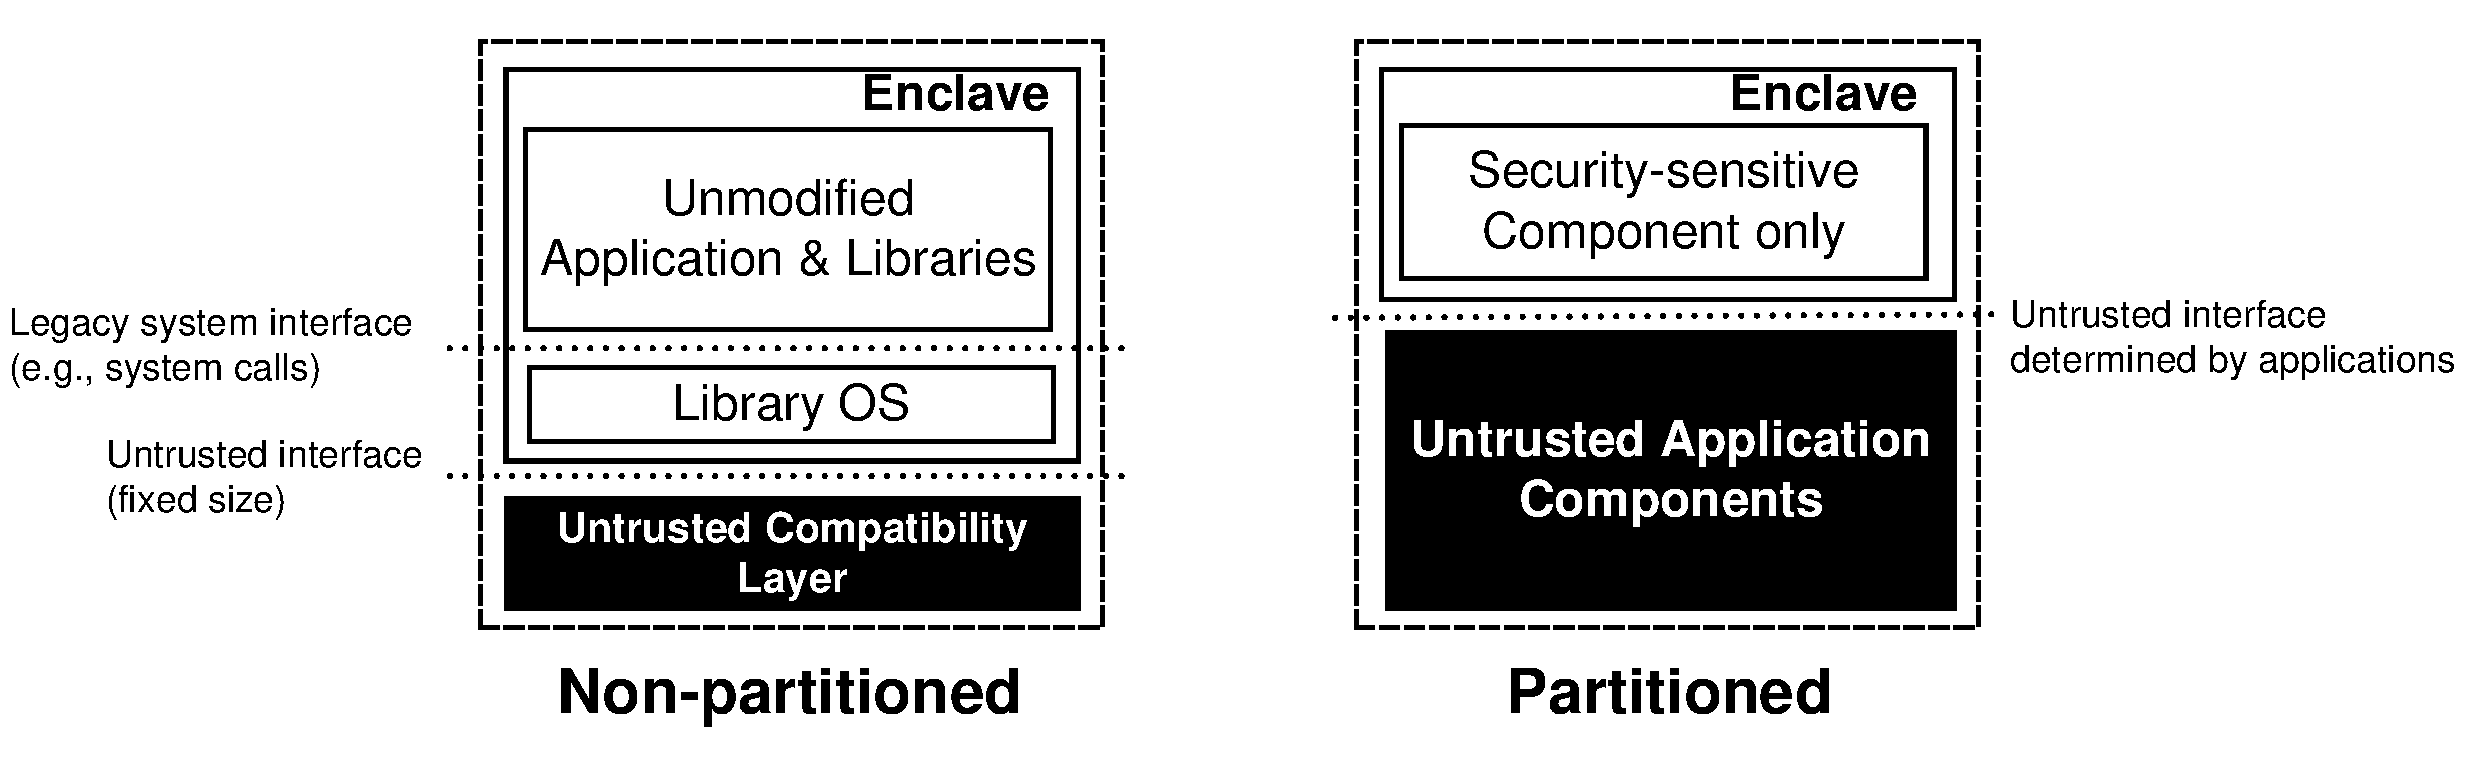
\includegraphics[width=5in]{graphene-sgx/figures/libosvssdk.pdf}
%\footnotesize
%\vspace{-0.3in}
%\caption[Comparison between libOS-based model and partitioned model for Intel SGX]
%{Comparison between libOS-based model (e.g., \haven{} and \sysname{})
%and SDK-based (SDK for \sgx{}) model for migrating applications in enclaves.
%Green (light) boxes are trusted components and red (dark) boxes are untrusted.
%The libOS-based model often yields a larger TCB in the enclave,
%while the SDK-based model requires developers to be responsible of
%securing the enclave on the untrusted interface.}
%\label{fig:libosvssdk}
%\end{figure}

\intel{} \sgx{} (Software Guard Extension)
is a set of new x86/x86\_64 instructions
introduced in the latest \intel{} \skylake{} processors,
to create, interface and attest
an isolated memory region (\emph{enclave}) inside applications' virtual memory.
\sgx{} guarantee any data in an enclave
stay encrypted in the DRAMs, using a secret key derived from
the application's cryptographic measurements.
The secret data store in the enclave memory
can only be accessed within the code inside the enclave,
and the code must be signed by the developers' private key.
The use cases of \sgx{} mostly involve an enclave
retrieving a signed attestation from the \intel{} processor,
to exchange provisioning of information from trusted remote servers.
The purpose is equivalent to
expanding the execution from remote servers
to untrusted hosts,
to securely harness resources such as CPU cycles and DRAMs.

\sgx{} is an appealing tool for protecting small, highly sensitive execution, 
against malicious or compromised OSes, hypervisors, or even hardware peripheral.
For instance, \cite{hoekstra13sgx} show how SGX can be used
to build a trusted path from a video chat application to a GPU and network card, which maintains confidentiality and integrity of the
video stream, even if the OS is compromised.
Similarly, because DRAM contents are encrypted, SGX can resist attacks such as cold-boot attacks~\cite{halderman09coldboot} or 
malicious peripheral devices~\cite{hudson15thunderstrike}.

\paragraph{A Partitioned Usage Model.}
To secure an application with \sgx{},
the common usage model requires the developers to partition the application into two parts:
the trusted part which runs the sensitive execution in the enclave,
and the untrusted part which loads and triggers the execution of the trusted parts.
%Developers shall keep the trusted path as small and simple
%Even if the trusted code only contains the simplest the logic,
%the untrusted code is still needed to pass the input and output of the execution.
The interaction between the trusted and untrusted parts is through \emph{untrusted interfaces}.
Untrusted interfaces are defined by the developers, and include a few
logical entry and exit points of the enclave.
In the architectural level,
an enclave only has exactly one hardware entry point and one exit point.
The architecture forbids the untrusted part
to willingly jump into any location of an enclave,
to bypass or alter the valid behavior of the trusted part.
The control flow of the execution is the enclave transfers to one of the logical entry points,
based on the input parameter passed
at the hardware entry point.
%The control transfer from the hardware entry point to the logical entry points
%is based on the operation code passed as an argument at enclave entry.

With the partitioned usage model,
the developers can minimize the trusted computing base (TCB) of the enclave,
at their best effort,
and restraint the behavior of the isolated execution.
% that can only be triggered by the untrusted interface.
The partitioning prevents unpredictable behaviors in the enclave,
to compromise the confidentiality or integrity.
The developers explicitly mark the sites in the application code
to determine entry and exit of the enclave.
%The untrusted and trusted code must explicitly call for enclave entry or exit
%at the fixed sites in the application.

%\intel{} \sgx{} ({\it Software Guard Extensions})
%are a set of new x86/x64 instructions
%introduced in the \intel{} Skylake processor family.
%Using \sgx{}, an 
%application can designate part of its virtual memory as an {\em enclave}.
%The CPU guarantees that the contents of the enclave never leave the CPU package unencrypted.
%The CPU also measures the integrity of a binary loaded into the enclave, and offers remote attestation,
%similar to a TPM~\cite{TPM}.


%%% create a protected memory region, called an {\em enclave}, inside it's virtual memory,
%%% where it can load its security sensitive data with hardware-enforced isolation from the untrusted OS. 
%%% The processor with \sgx{}
%%% guarantees that any data loaded in enclave
%%% stays encrypted in the DRAM, by using a secret key deterministically derived from the application's cryptographic measurement and the CPU secret. 



% \sgx{} provides useful building blocks for secure applications, but does not
%absolve the programmer of all responsibility for reasoning about end-to-end security.
%Bugs in the application or supporting libraries can still disclose sensitive data from an enclave,
%and porting code into SGX can be subtle.
%
%Fundamentally, this argues for writing enclave code in higher-level languages
%(e.g., \java{}) that provide important 
%safety properties, such as memory and type safety, that reduce or eliminate common vulnerabilities.
%Ideally, one would formally verify security properties of enclave code~\cite{moat}; this verification is significantly aided by using 
%higher-level languages amenable to formal reasoning.  Verification is significantly harder
%with C/C++ or assembly languages.

%One must note that \sgx{} only promises the integrity of application binaries
%initially loaded in enclaves.
%The gap between integrity of binaries and complete security has to be filled
%by ones who develop and approve the applications.
%More specifically, the clients are responsible of
%testing whether the applications contain any vulnerabilities
%that lead to information leak.
%To minimize the risk of leaving any flaws in the applications unintentionally,
%developers often tend to cut down the trusted computing base (TCB)
%of the applications. With smaller TCB, clients who launched the enclaves
%can more easily reason about the thoroughness of securing the execution.

%To achieve smaller TCB, the software development kit of \sgx{}
%intends to encourage developers to partition the applications and
%keep only security sensitive components in the enclaves.
%Such an intention is exactly contradicted by the trust model of \haven{},
%which must trust the loaded application as a whole.
%Except for the cases in which the whole applications must be secured,
%\haven{} actually downgrades the trustworthiness of enclaves.
%Figure~\ref{fig:gsgx:libosvssdk} shows the comparison of the two models.

\paragraph{Using A Library OS.}
 
The partitioned usage model
restricts the risk of the isolated execution being
compromised by the untrusted host,
yet requires the developers to
cleanly split a part of the application
and inject entry and exit points at wherever interaction is needed.
Moreover, the developers are responsible
for validating and examining the soundness of the partitioned application,
to ensure every execution paths in the enclave
that are affected by the untrusted entities
are carefully checked and sanitized.
Porting a legacy application to a partitioned model
requires developers to have substantial familiarity to the application code,
as well as the principles for
developing unexploitable,
well-controlled execution in the enclave.
%be familiar with
%the mechanism of enclave entry and exit,
%and always bear the security of the isolated execution in mind.
%For developers that are not expert to architecture and security issues,
%pursuing the partitioned model may need significant efforts.   
When the sensitive execution to be isolated in the enclave
becomes considerably complex,
the effort for porting and validating the execution
quickly becomes unacceptably expensive.

\emph{Haven}~\cite{baumann14haven}
shows a \emph{non-partitioned usage model},
for loading whole, unmodified applications and supporting libraries
into enclaves.
The non-partitioned model allows application to be run in the enclave as it is, without any porting effort.
To support the non-partitioned model,
a key requirement is to support the system APIs needed by
the application and supporting libraries,
right inside the enclave.
Essentially, the execution not only is forbidden to access any host system APIs
(i.e., using {\tt syscall} or {\tt sysenter} instructions)
in the enclave,
but also unsafe to rely on the untrusted host
to provide system APIs.
A \libos{}, on the other hand, supports system APIs as in-memory function calls,
and mediates all input and output
during interaction with the untrusted host.
For instance, Haven supports unmodified Windows applications in enclaves,
using \drawbridge{} \libos{}~\cite{porter11drawbridge}
to handle all the Windows API calls.

At the low level, the non-partitioned model still requires partitioning, but instead of the applications,
it is the \libos{} itself that needs to be partitioned.
More precisely, The \pal{} that provides host ABI to the \libos{} is the component that is split across the two sides of the enclave boundary,
while the \libos{}, alone with the isolated application
and its supporting libraries,
are dynamically loaded.
The partitioned \pal{} interacts with the host through a fixed, narrow untrusted interface,
to access host resources if necessary.
%interacts with a \libos{}-specific untrusted interface,
%which is the only trusted interface needed to be defined,
%and will never be extended no matter which application is loaded.


\subsection{Porting \graphene{} to \intel{} \sgx{}}

\fixme{Need transition here}

The building blocks are shown as figure~\ref{fig:graphene:sgx-arch}.
\graphenesgx{} is partitioned into two parts:
an untrusted \pal{} to initialize the enclave and provide the untrusted interface;
and the trusted \libos{} including the host ABI, {\tt libLinux}, and core {\tt libc} libraries.
Except the host ABI is statically loaded in the enclave since the start up,
other components of \graphenesgx{} in the enclave are dynamically loaded,
as needed. 
%For each binary loaded by \sysname{}, \sysname{} bootstraps the enclave
%from an untrusted platform adaption layer (PAL) that defines
%a narrowed untrusted interface.
%To speed up initialization, the untrusted PAL starts the enclave
%with an statically linked library image ({\tt graphene.so}).
%The image includes
%\graphene{} host ABI,
%\libos{} ({\tt libLinux}, implementing Linux personality),
%and basic libraries of GNU library C
%({\tt libc}, {\tt libpthread} and {\tt ld}, the runtime loader).
%The \sysname{} library image then loads the unmodified applications
%and libraries into the enclave.
After the \libos{} is laoded in the enclave,
the \libos{} will load the application and its supporting libraries,
and call their entry functions.
The \libos{} will handle all the system calls redirected from the applications,
whereas it may access host resource through the host ABI calls,
which are redirected to the untrusted interface
to interact with the host. 

\begin{figure}[t!]
\centering
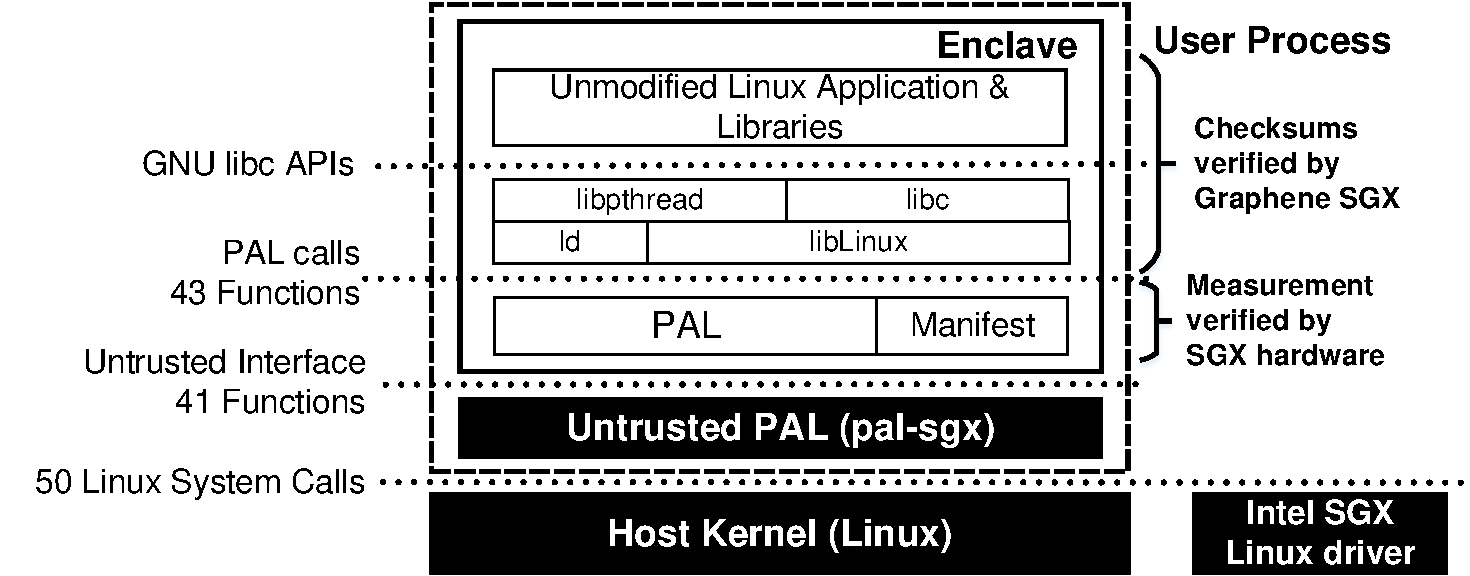
\includegraphics[width=5.5in]{graphene-sgx/figures/architecture.pdf}
\footnotesize
\caption[The \graphenesgx{} building blocks]
{The \graphenesgx{} building blocks.
Green (light) boxes are trusted components trusted,
and red (dark) boxes are untrusted.
\graphenesgx{} is statically linked with {\tt libLinux},
the \libos{} binary, and basic libraries of GNU library C.
To build up the trust, the \graphenesgx{} image along with
a manifest and application measurements
are verified by \sgx{} during bootstrap. Applications and other libraries
are verified by \graphenesgx{}. The enclave interacts with the host kernel,
through untrusted PAL, on a narrowed untrusted interfaces with 41 functions.}
\label{fig:graphene:sgx-arch}
\end{figure}

\paragraph{Applications Integrity.}
A key requirement of the non-partitioned usage model is to guarantee the integrity of the secured applications.
Because the applications are dynamically loaded by the \libos{}
{\em after} the enclave starts up,
the CPUs cannot verify the integrity of loaded application binaries.
An alternative is to place all application binaries in an encrypted virtual disk,
which can be decrypted using a securely provisioned key~\citep{baumann14haven}.

\graphenesgx{} guarantees the integrity of applications
by signing each supporting binaries or generating checksums for the binaries.
For each secured application, the signing tool will generate
a manifest and a correspondent signature.
A manifest will contain the attributes of the enclave and \libos{},
and the checksums of the supporting binaries.
The manifest will be loaded in the enclave before the enclave starts,
and verified by the hardware as part of the enclave measurement.
The integrity of the supporting binaries
are validated by \pal{} before loading from the untrusted host.

By verify the integrity of applications individually,
we decouple the deployment and verification of the application binaries;
users may simply deploy the manifest and the signature to the untrusted host,
and all the binaries, including the \libos{}, can be loaded from the local file system.

\paragraph{Untrusted Interface.}
The untrusted interface is defined as Table~\ref{tab:graphene:sgx-interface}.
\graphenesgx{} draws the untrusted interface right above the calling
of the host APIs (Linux system calls) in \pal{}.
Most code inherited from the \graphene{} Linux \pal{} stays in
the enclave, to keep the states secure.
Because the host is not trusted,
\graphenesgx{} is built upon the assumption that the untrusted interface
can be exploited to
pass malicious arguments, or return incorrect results.
For example, {\tt file\_open} may return a file descriptor that points
to a wrong file, or {\tt map\_untrusted} may return an address in the enclave. 
Beside checking for malicious returned results,
\graphenesgx{} must actively check the behavior of the host.

For instance, if the isolated application opens a stream for IO,
\graphenesgx{} must guarantee either the stream is protected cryptographically,
or assume that nothing is safely read or written.
In addition, \graphenesgx{} does not include {\tt file\_sync} in the untrusted interface,
because it does not trust the host to faithfully flush any stream.
With a robustly designed untrusted interface,
the worst scenario a malicious host can cause is \term{denial-of-the-service}.

%The Untrusted interface of an enclave is the API that communicates the enclave
%and the untrusted host, with both entries and exits of the enclave.
%Note that for hardware an enclave only has exactly one entry and exit,
%to which execution jumps
%using {\tt EENTER} and {\tt EEXIT} instructions.
%The untrusted interface is simply a callback table that redirects execution
%afterward (similar to system calls).

\begin{table}[t!]
\centering
\footnotesize
\begin{tabular}{lc>{\palign[\tt]{l}}p{4.5in}}
\hline
\addlinespace
Classes & \# & {\normalfont\bf Untrusted Interface Functions} \\
\addlinespace
\hline
Entries / Exits & 3 & 
start\_enclave
exit\_enclave
start\_thread
\\
\hline
Memory & 2 &
map\_untrusted
unmap\_untrusted
\\
\hline
Scheduling & 4 &
sleep
schedule
futex
gettime
\\
\hline
Cloning & 2 &
clone\_thread
clone\_process
\\
\hline
Files & 8 &
file\_open
file\_mkdir
file\_rename
file\_delete
file\_truncate
file\_write
file\_read
file\_readdir
\\
\hline
Sockets & 8 &
sock\_listen
sock\_accept
sock\_connect
socketpair
sock\_send
sock\_receive
sock\_shutdown
sock\_setopt
\\
\hline
File Descriptors & 3 &
fd\_close
fd\_size
fds\_poll
\\
\hline
Misc & 3 &
print\_debug
load\_gdb
cpuid
\\
\hline
\end{tabular}

\caption[The \graphenesgx{} untrusted interface]
{The \graphenesgx{} untrusted interface, which consists of \interfacenum{} functions in total.
Most of the interface is derived from the host system call footprint of
\graphene{} \libos{}. Enclave must not trust the hosts to
always return right responses or faithfully perform operations.}
\label{tab:graphene:sgx-interface}
\end{table}

%\paragraph{The Signing Tool.}
%Each enclave launched in \sgx{} requires a signature, signed by the developers' private key.
%The signature structure ({\tt SIGSTRUCT}) contains
%the enclave attributes, product ID, the enclave measurement,
%and RSA-based signature of the structure.
%\sysname{} maintains enclave signatures on a per-binary basis.
%Unlike \haven{}, we extend the enclave's measurement to
%cover all binaries loaded in the enclave, not just the \libos{} itself.
%To keep the application binaries being dynamically loaded,
%the measurement of these binary files are stored as
%{\bf application checksums}, verified by \sysname{} at loading.
%With the application checksums being measured in enclaves,
%different binaries loaded with different library dependencies
%will naturally yield different measurements,
%easily differentiating the attestations generated by processors.

\paragraph{Signing and Launching Applications.}
A key requirement of supporting the non-partitioned model is to secure the process of dynamic loading.
In \graphenesgx{}, application binaries are verified by their checksums.
The enclave manifest lists all the checksums,
and is included in the cryptographic measurement when the enclave starts.
The measurement for launching the enclave is distinct
for different applications.

When developers port an application to \graphenesgx{},
the enclave signature are generated by the signer,
on a trusted host.
The signing process essentially creates a snapshot of
the trusted execution environment,
by hashing all the binaries to be loaded.
After the signing, developers ship the application, along side with the enclave signature, manifest, \graphenesgx{} binaries and all the supporting libraries,
to the untrusted hos,
on which \graphenesgx{} loads the application in the enclave.

%where applications are loaded,
%an architectural enclave called {\tt aesm} on each platform that supports \sgx{}
%must be trusted by all enclave.
%{\tt aesm} is a secured service signed by \intel{} for generating
%valid enclave tokens.
%The {\tt aesm} binary is part of the \sgx{} SDK,
%and signed using an \intel{} internal key, thus cannot be
%tampered by any third party.
%Otherwise, any other parts of the platform that launches the enclave
%must not be trusted, including the host kernel,
%\sgx{} kernel driver, and most parts of the hardware except the processor.

%Although \haven{} only includes the shielding module
%in the enclave measurements,
%it can still differentiate applications by forcing different digests
%on the same shielding module.
%The trick is to inject an unique ID for each application,
%into the module binary.
%We argue that \sysname{} uses a more straightforward model, with no need to
%maintain the uniqueness of any IDs.
%
%
%
%
%
%
%
%However, carefully engineering the untrusted interface is simply not enough
%to secure the enclave.
%We must not rely on the applications to always
%sanitize IO or encrypt the streams,
%especially if the applications are formally assumed to run on trusted host.
%\sysname{} requires clients to provide {\bf manifests} to state
%the policy of applications while accessing the untrusted interface.
%The manifests are measured, so their integrity can be attested by processors.
%For example, all streams opened must be either encrypted or signed,
%unless the manifest explicitly states ones as unimportant
%(e.g., debug streams).
%Another type of policies can be used for authenticate other ends of RPC streams
%based on the measurements of target enclaves.
%These policies are used to decentralize the trust in multi-process applications,
%that we will discuss in length in section~\ref{sec:multiproc}.

\paragraph{Threat model.}
The host ABI, \libos{}, {\tt libc} and all supporting libraries and binaries
that loaded into the enclave
must be considered as part of the TCB.
The rest of system, including the untrusted \pal{}, the host, any hardware peripheral or remote entity that are not attested
can be malicious or compromised
to launch arbitrary attack on the isolated application.
%When an application is loaded by \sysname{}, it ought to be trusted by
%certain remote entities
%for provisioning confidential information or
%accepting the enclave's computation results.
%The trusted application code in the enclave includes both
%{\bf static} and {\bf dynamic} parts.
%The host ABI, library OS, and basic GNU lib C are loaded statically
%at the enclave launching time,
%with their integrity verified by the processor.
%Otherwise, any code that is dynamically loaded, or generated at runtime
%(e.g., by just-in-time compilation),
%must be secured by \sysname{} or other trusted parts.
For multi-process applications, each \picoproc{} created by \graphenesgx{}
will be isolated in its own enclave.
No mutual trust is required between the \picoprocs{},
unless the \term{manifest file}
allows sharing the multi-process abstractions.
%For example, a parent process can decide to pass output to a child process
%through a secured pipe,
%but the parent process does not have to trust the child, assuming
%the parent will sanitize any information passed to the child.
%For processes that have the same security level,
%clients can also put them into a mutually trusted group,
%where all processes are allowed to share any abstractions.

\paragraph{Side-Channel Attacks.}
We consider side-channel attacks as a potential threat in \graphenesgx{}.
%Since enclaves are launched on untrusted hosts, it is hard to prevent
%enclaves from becoming vulnerable to side-channel attacks.
Attackers may exploit timing channels to expose confidential
information in the enclave, and current \sgx{} technology has no defense
against these attacks.
\cite{xu15controlledchannel} show a stronger attack than regular side-channel attacks, as \term{controlled channel attacks}.
This type of attack exploits the fact that an enclave must cooperate
with the host OS for page management,
the OS can manipulate paging to amplify the side channels
for exposing more secrets.
%Currently there is no defense against this type of attacks, except minimizing
%the side channels by rearranging code and data in enclave pages.
Both side-channel attacks and Controlled channel attacks
are common problems in all solutions based on \sgx{},
including \haven{}. In this paper, we consider solving these attacks as
out of the scope to our work.

%\paragraph{Remote attestation.}
%For enclaves, the only way to be securely provisioned by another entity
%is by attestation.
%\sgx{} provides a signed proof of the enclave measurement,
%which can be verified by other entities as long as their platforms
%also support \sgx{}.
%In \haven{} model, the same shielding module cannot have different applications
%securely provisioned, because their enclave measurements will simply
%appear no difference.
%Because \sysname{} includes the applications into enclave measurements,
%\sgx{} can generate attestation that differentiates the loaded applications.



